% !TEX program = xelatex
\documentclass[11pt,a4paper]{article}

% =====================================================================================================
%  Sample Article: "Adaptive Sampling for Sparse Signal Recovery"
%  ILLUSTRATIVE TEMPLATE. The model, data, tables and figures come from a small synthetic simulation
%  (see figures/generate_sample_article_figures.py). They are NOT findings of real research.
%  Customize: title/author (below), palette (Theme colors), fonts (Fonts), page size (geometry).
%  Figures are plain PDFs in figures/ (extension-less \includegraphics): replace the files, keep the names.
% =====================================================================================================

% ---- Packages ----
\usepackage{fontspec}
\usepackage[a4paper,margin=2.5cm]{geometry}   % CUSTOMIZE: page size and margins
\usepackage{amsmath,amssymb,amsthm}
\usepackage{graphicx}
\usepackage{booktabs}
\usepackage{enumitem}
\usepackage{microtype}
\usepackage{xcolor}
\usepackage{sectsty}
\usepackage[font=small,labelsep=period,skip=6pt]{caption}
\usepackage{algorithm}
\usepackage{algpseudocode}
\usepackage{hyperref}

% ---- Fonts ----
\setmainfont{TeX Gyre Termes}   % primary text face (bundled with Plum)
% Complementary sans for headings, captions and table heads. TeX Gyre Heros is used when installed;
% otherwise the bundled Termes (bold) is used, so the document always compiles. CUSTOMIZE: swap the family names.
\IfFontExistsTF{TeX Gyre Heros}{\newfontfamily\lpHeadingFont{TeX Gyre Heros}}{\newfontfamily\lpHeadingFont{TeX Gyre Termes}}

% ---- Theme colors ----
% Restrained scientific palette: deep navy (accent, links, section titles), teal (subsections), near-black text.
\definecolor{lpAccent}{HTML}{1F3A5F}
\definecolor{lpBody}{HTML}{1A1A1A}
\definecolor{lpSection}{HTML}{1F3A5F}
\definecolor{lpSubsection}{HTML}{2E7D8C}
\AtBeginDocument{\color{lpBody}}
\hypersetup{colorlinks=true,linkcolor=lpAccent,citecolor=lpAccent,urlcolor=lpAccent}
\sectionfont{\lpHeadingFont\color{lpSection}}
\subsectionfont{\lpHeadingFont\color{lpSubsection}}

% ---- Supporting palette (notice box, captions, metadata) ----
\definecolor{lpMuted}{HTML}{5B6573}
\definecolor{lpTint}{HTML}{EEF2F6}

% ---- Layout and typography ----
\setlist{nosep,leftmargin=*,itemsep=2pt,topsep=4pt}
\setlength{\parindent}{1.4em}
\setlength{\emergencystretch}{2em}
\renewcommand{\arraystretch}{1.15}
\DeclareCaptionFont{lpHead}{\lpHeadingFont}
\captionsetup{labelfont={bf,lpHead}}
\captionsetup[table]{position=above}
\theoremstyle{definition}
\newtheorem{problem}{Problem}

% ---- Notation ----
\DeclareMathOperator{\supp}{supp}
\newcommand{\R}{\mathbb{R}}
\newcommand{\E}{\mathbb{E}}
\newcommand{\norm}[1]{\lVert #1\rVert}

% ---- Helpers: remove the notice and \illus when you replace the simulated content with real results ----
\newcommand{\illus}{\textit{Illustrative simulation.}\ }
\newcommand{\thead}[1]{\textbf{\lpHeadingFont #1}}
\newcommand{\keywords}[1]{\par\smallskip\noindent{\lpHeadingFont\bfseries Keywords:}\ #1\par}
\newcommand{\illustrativenotice}[1]{\par\medskip\noindent\colorbox{lpTint}{\parbox{\dimexpr\linewidth-2\fboxsep\relax}{\small\color{lpMuted}#1}}\par\bigskip}

% Title block and abstract styling
\makeatletter
\providecommand{\and}{\end{tabular}\hskip 1.5em\begin{tabular}[t]{c}}
\renewcommand{\maketitle}{%
  \begin{center}
    {\lpHeadingFont\bfseries\LARGE\color{lpAccent}\@title\par}\vspace{1.2em}
    {\large\begin{tabular}[t]{c}\@author\end{tabular}\par}\vspace{0.8em}
    {\small\color{lpMuted}\@date\par}
  \end{center}\par\vspace{0.2em}}
\makeatother
\renewenvironment{abstract}{%
  \begin{list}{}{\setlength{\leftmargin}{1cm}\setlength{\rightmargin}{1cm}\setlength{\listparindent}{0pt}\setlength{\parsep}{0pt}}%
  \item\relax{\lpHeadingFont\bfseries\color{lpAccent}\abstractname.}\ \small}{\end{list}}

% ---- Title and authors (placeholders) ----
\title{Adaptive Sampling for Sparse Signal Recovery\\[0.4em]{\large\mdseries A Multi-Stage Measurement Design}}
\author{First Author\\{\small Department, Institution}\\{\small\texttt{first.author@example.org}}
  \and Second Author\\{\small Department, Institution}\\{\small\texttt{second.author@example.org}}}
\date{\today}

\begin{document}
\maketitle

\begin{abstract}
Sparse signals can be recovered from far fewer linear measurements than their ambient dimension, but the
measurements themselves are usually fixed in advance. We ask whether choosing them adaptively helps.
We formulate a multi-stage design in which each stage concentrates its sensing energy on a candidate support
estimated from earlier stages, and recover the signal by $\ell_1$-regularised least squares followed by
support debiasing. In a synthetic study ($n=256$, $s=8$, 300 trials per setting), a three-stage design with
$m=80$ measurements reaches a median relative error of $0.032$, against $0.061$ for non-adaptive Gaussian
sampling, and recovers the support exactly in $97.0\%$ of trials against $92.7\%$. With $m=48$ the advantage
disappears because the first stage is too small to localise the support. All numbers are illustrative simulation
output that demonstrates this template.
\keywords{adaptive sampling; compressed sensing; sparse recovery; sequential experimental design; LASSO}
\end{abstract}

\illustrativenotice{\textbf{Illustrative document.} The data model, simulation results, tables and figures below are
synthetic and exist to demonstrate the template (equations, algorithm, tables, figures and citations). They are not
real research findings. The cited works are real and listed for context only; verify each entry before reuse.}

% ===================================================================================================
\section{Introduction}\label{sec:intro}

\subsection{Background and motivation}\label{sec:background}
Compressed sensing recovers signals from \textbf{far fewer samples} than classical theory requires, provided the signal is
sparse in a known basis~\cite{candes2006,donoho2006,foucart2013}. In the standard setting the measurement vectors are drawn at random
and never revisited. Many practical instruments are sequential, however: each measurement can be chosen after the previous
ones have been read. A scanning microscope, a spectrum sensor or a field survey can all spend later measurements where
earlier ones indicate that the signal lives. Two observations motivate this paper:
\begin{itemize}
  \item sparse priors and \textbf{basis pursuit} make a rough support estimate cheap to obtain from few measurements;
  \item \textit{adaptive} measurement schedules can turn that estimate into higher sensing energy where it matters~\cite{haupt2011,ji2008}.
\end{itemize}

\subsection{Contributions and outline}\label{sec:contrib}
We keep the setting deliberately simple and make three contributions.
\begin{enumerate}
  \item A budgeted multi-stage sampling problem with an explicit per-measurement energy constraint (Section~\ref{sec:problem}).
  \item A practical algorithm that alternates LASSO estimation and support refinement (Algorithm~\ref{alg:adaptive}).
  \item An illustrative simulation comparing adaptive and non-adaptive strategies (Section~\ref{sec:results}).
\end{enumerate}
Section~\ref{sec:problem} states the problem, Section~\ref{sec:method} the method, Section~\ref{sec:results} the results,
and Sections~\ref{sec:discussion}--\ref{sec:conclusion} discuss limits and conclusions.

% ===================================================================================================
\section{Problem formulation}\label{sec:problem}

\subsection{Measurement model}
Let $x\in\R^n$ be an unknown $s$-sparse signal, $\norm{x}_0\le s$ with support $T=\supp(x)$. We observe $m$ noisy linear measurements
\begin{equation}\label{eq:model}
  y_i = \langle a_i, x\rangle + \varepsilon_i,\qquad \varepsilon_i\sim\mathcal N(0,\sigma^2)\ \text{i.i.d.},\quad i=1,\dots,m,
\end{equation}
or $y = Ax + \varepsilon$ in matrix form, where the rows of $A$ are the sensing vectors $a_i$. The classical estimator is the LASSO~\cite{tibshirani1996},
\begin{equation}\label{eq:lasso}
  \hat{x} = \arg\min_x \tfrac{1}{2}\lVert y - Ax \rVert_2^2 + \lambda \lVert x \rVert_1 ,
\end{equation}
with regularisation parameter $\lambda>0$. Its performance depends on how much sensing energy reaches the coordinates in $T$.

\subsection{Adaptive design}
The measurements are collected in $K$ stages. Stage $k$ takes $m_k$ measurements with index set $\mathcal I_k$, $\sum_k m_k=m$. Let $\mathcal S_0=\{1,\dots,n\}$ and let $\mathcal S_k\subseteq\mathcal S_{k-1}$ be the candidate set formed after stage $k$. Rows in stage $k$ are Gaussian and live on the previous candidate set,
\begin{equation}\label{eq:rows}
  a_i\sim\mathcal N\!\Bigl(0,\ \tfrac{1}{|\mathcal S_{k-1}|}\operatorname{diag}\bigl(\mathbf 1_{\mathcal S_{k-1}}\bigr)\Bigr),\qquad i\in\mathcal I_k,
\end{equation}
so that $\E\norm{a_i}_2^2=1$ in every stage: adaptivity \emph{redistributes} a fixed energy budget, it never enlarges it.
The expected sensing energy delivered to coordinate $j$ is
\begin{equation}\label{eq:energy}
  E_j=\sum_{k=1}^{K}\frac{m_k}{|\mathcal S_{k-1}|}\,\mathbf 1\{j\in\mathcal S_{k-1}\},
  \qquad E_j^{\text{non-adaptive}}=\frac{m}{n}.
\end{equation}

\subsection{Research problem}
\begin{problem}[Budgeted adaptive recovery]\label{prob:main}
Given $n$, $s$, $\sigma$, a budget of $m$ unit-energy measurements and the model~\eqref{eq:model}, choose the stage sizes $(m_k)$, the candidate sizes $(c_k)=(|\mathcal S_k|)$ and the data-dependent rows~\eqref{eq:rows} to minimise the expected relative error
\begin{equation}\label{eq:objective}
  \min_{(m_k),(c_k)}\ \E\bigl[\rho(\hat x,x)\bigr],\qquad
  \rho(\hat x,x)=\frac{\norm{\hat x-x}_2}{\norm{x}_2},\qquad \text{s.t. } \sum_{k=1}^{K}m_k=m .
\end{equation}
\end{problem}
We study three research questions:
\begin{enumerate}[label=\textbf{RQ\arabic*.}]
  \item Does concentrating energy on a candidate support reduce error at equal total energy?
  \item How many stages are useful?
  \item What is the smallest budget $m$ at which adaptivity pays off?
\end{enumerate}

% ===================================================================================================
\section{Methodology}\label{sec:method}

\subsection{Estimation, candidate update and debiasing}
After each non-final stage, all data collected so far are fed to the LASSO~\eqref{eq:lasso} with columns normalised to unit norm and
\begin{equation}\label{eq:lambda}
  \lambda=\kappa\,\sigma\sqrt{2\ln n},
\end{equation}
a standard noise-level choice with a constant $\kappa$. The next candidate set keeps the $c_k$ coordinates with the largest estimated magnitude,
\begin{equation}\label{eq:candidate}
  \mathcal S_k=\{\text{the } c_k \text{ indices with largest } |\hat x^{(k)}_j|\}.
\end{equation}
After the last stage, the $s$ largest entries define $\hat T$ and the final estimate removes the LASSO shrinkage by least squares on that support,
\begin{equation}\label{eq:debias}
  \hat x=\arg\min_{z:\ \supp(z)\subseteq\hat T}\ \norm{y-Az}_2^2 .
\end{equation}
Algorithm~\ref{alg:adaptive} summarises the procedure.

\begin{algorithm}[tbp]
\caption{Multi-stage adaptive sampling with LASSO refinement}\label{alg:adaptive}
\begin{algorithmic}[1]
\Require $n,\ s,\ \sigma$; stage sizes $(m_k)_{k=1}^K$; candidate sizes $(c_k)_{k=1}^{K-1}$; constant $\kappa$
\Ensure estimate $\hat x$
\State $\mathcal S_0\gets\{1,\dots,n\}$,\quad $\lambda\gets\kappa\,\sigma\sqrt{2\ln n}$ \Comment{Eq.~\eqref{eq:lambda}}
\For{$k=1,\dots,K$}
  \State draw $m_k$ rows on $\mathcal S_{k-1}$ by~\eqref{eq:rows}; measure; append to $(A,y)$
  \If{$k<K$}
    \State $\hat x^{(k)}\gets$ LASSO$(A,y,\lambda)$ \Comment{Eq.~\eqref{eq:lasso}}
    \State $\mathcal S_k\gets$ indices of the $c_k$ largest $|\hat x^{(k)}_j|$ \Comment{Eq.~\eqref{eq:candidate}}
  \EndIf
\EndFor
\State $\hat x^{(K)}\gets$ LASSO$(A,y,\lambda)$;\quad $\hat T\gets$ indices of the $s$ largest $|\hat x^{(K)}_j|$
\State \Return $\hat x\gets$ least squares on $\hat T$ \Comment{Eq.~\eqref{eq:debias}}
\end{algorithmic}
\end{algorithm}

\subsection{Why energy concentration should help}
Once the candidate set contains $T$, the rows of every stage are isotropic on $T$ and $A_T^{\top}A_T\approx \bar E\,I$ with $\bar E=E_j$ for $j\in T$ from~\eqref{eq:energy}. Least squares on the support then gives the heuristic
\begin{equation}\label{eq:var}
  \operatorname{Var}(\hat x_j)\approx\frac{\sigma^2}{E_j}
  \quad\Longrightarrow\quad
  \rho\approx\frac{\sigma\sqrt{s/\bar E}}{\norm{x}_2},
\end{equation}
which ignores support errors and the dependence between stages. It is a design guide, not a theorem. For the budget used below ($m=80$, stages $40/20/20$, candidate sizes $64$ and $24$), Eq.~\eqref{eq:energy} gives $\bar E=40/256+20/64+20/24\approx1.30$ against $80/256\approx0.31$ for non-adaptive sampling, a $4.2\times$ gain; the best conceivable value, with the support known in advance, is $m/s=10$.

% ===================================================================================================
\section{Illustrative results}\label{sec:results}

\subsection{Simulation setup}
Table~\ref{tab:setup} lists the synthetic setup. Signals, noise and sensing matrices are drawn at random; the four strategies are compared on the same signals. The \emph{oracle} knows $T$ and senses only on it, which is the best any strategy can achieve under the energy constraint.

\begin{table}[tbp]
\centering
\caption{\illus Simulation parameters.}\label{tab:setup}
\small
\begin{tabular}{@{}ll@{}}
\toprule
\thead{Quantity} & \thead{Value} \\
\midrule
Ambient dimension, sparsity & $n=256$, $s=8$ \\
Non-zero amplitudes & $|x_j|\sim\mathrm U[1,2]$, random signs \\
Noise level & $\sigma=0.05$ \\
Budgets & $m\in\{48,64,80,96,112,128\}$ \\
Two-stage design & $m_1/m=0.6$, $c_1=48$ \\
Three-stage design & $m_k/m=0.50,\,0.25,\,0.25$, $(c_1,c_2)=(64,24)$ \\
Solver & FISTA~\cite{beck2009}, 400 iterations, $\kappa=1.6$ in~\eqref{eq:lambda} \\
Replications & 300 per $(m,\text{strategy})$ \\
\bottomrule
\end{tabular}
\end{table}

\subsection{Adaptive-sampling behaviour}
Figure~\ref{fig:curve}(a) shows how the three-stage design narrows the search. The candidate set shrinks from $256$ to $64$ to $24$ coordinates while the mean recall of the true support stays high ($0.94$ for $\mathcal S_1$, $0.98$ for $\mathcal S_2$). Figure~\ref{fig:curve}(b) shows the resulting energy allocation in one run: the coordinates that survive both rounds receive several times the energy of the rest.

\begin{figure}[tbp]
  \centering
  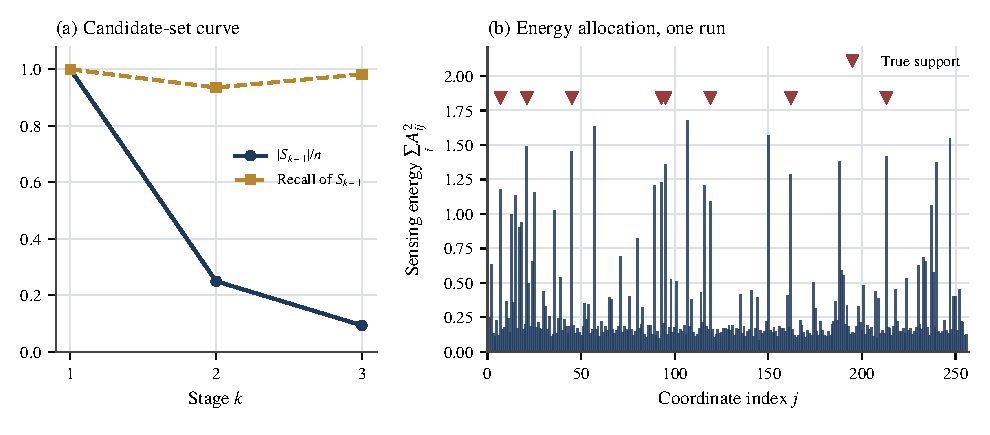
\includegraphics[width=\linewidth]{figures/adaptive-curve}
  \caption{\illus Adaptive sampling at $m=80$. (a) Candidate fraction $|\mathcal S_{k-1}|/n$ used by stage $k$ and mean recall of the true support, averaged over 300 trials. (b) Sensing energy $\sum_i A_{ij}^2$ per coordinate in a single run; triangles mark the true support.}\label{fig:curve}
\end{figure}

\subsection{Comparison of sampling strategies}
Figure~\ref{fig:recovery} compares the strategies: the relative error~\eqref{eq:objective} falls for every strategy as the budget grows, and the adaptive designs lie below the non-adaptive one from $m=64$ onwards. At $m=80$ the three-stage design halves the median error (Table~\ref{tab:results}), and Eq.~\eqref{eq:var} with $\norm{x}_2\approx4.3$ predicts $0.059$, $0.029$ and $0.010$ for the non-adaptive, three-stage and oracle strategies against the measured medians $0.061$, $0.032$ and $0.010$.

\begin{figure}[tbp]
  \centering
  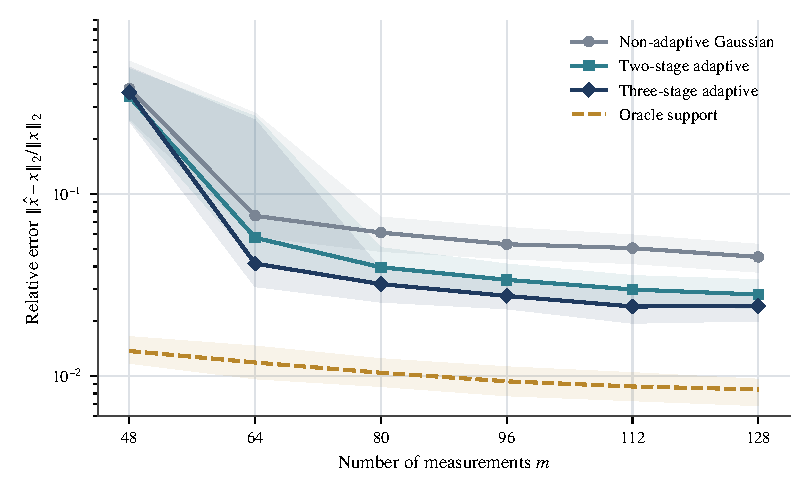
\includegraphics[width=0.85\linewidth]{figures/recovery}
  \caption{\illus Median relative error $\norm{\hat x-x}_2/\norm{x}_2$ versus the number of measurements $m$ (log scale). Shaded bands show the interquartile range over 300 trials.}\label{fig:recovery}
\end{figure}

\begin{table}[tbp]
\centering
\caption{\illus Recovery at $m=80$ (300 trials). Error: median [interquartile range]; $F_1$: mean support $F_1$ score; Exact: share of trials with $\hat T=T$.}\label{tab:results}
\small
\begin{tabular}{@{}lccc@{}}
\toprule
\thead{Strategy} & \thead{Relative error} & \thead{$F_1$} & \thead{Exact (\%)} \\
\midrule
Non-adaptive Gaussian & $0.061$ [$0.048$, $0.075$] & $0.990$ & $92.7$ \\
Two-stage adaptive    & $0.040$ [$0.032$, $0.051$] & $0.990$ & $92.3$ \\
Three-stage adaptive  & $\mathbf{0.032}$ [$0.025$, $0.039$] & $\mathbf{0.996}$ & $\mathbf{97.0}$ \\
\midrule
Oracle support        & $0.010$ [$0.009$, $0.012$] & $1.000$ & $100.0$ \\
\bottomrule
\end{tabular}
\end{table}

\begin{table}[tbp]
\centering
\caption{\illus Median relative error as a function of the budget $m$.}\label{tab:sweep}
\small
\begin{tabular}{@{}lcccccc@{}}
\toprule
\thead{Strategy} & \thead{$m=48$} & \thead{64} & \thead{80} & \thead{96} & \thead{112} & \thead{128} \\
\midrule
Non-adaptive Gaussian & $0.379$ & $0.076$ & $0.061$ & $0.053$ & $0.050$ & $0.045$ \\
Two-stage adaptive    & $0.343$ & $0.057$ & $0.040$ & $0.034$ & $0.030$ & $0.028$ \\
Three-stage adaptive  & $0.362$ & $0.041$ & $0.032$ & $0.028$ & $0.024$ & $0.024$ \\
Oracle support        & $0.014$ & $0.012$ & $0.010$ & $0.009$ & $0.009$ & $0.008$ \\
\bottomrule
\end{tabular}
\end{table}

\subsection{Resulting measurements}
Figure~\ref{fig:measurements}(a) lists the measurements of a single three-stage run. The later stages, taken on small candidate sets, show larger magnitudes because each of them concentrates its unit energy on few coordinates. Figure~\ref{fig:measurements}(b) compares the recovered and true coefficients on the support for the same signal: the relative errors are $0.073$ (non-adaptive) and $0.023$ (three-stage).

\begin{figure}[tbp]
  \centering
  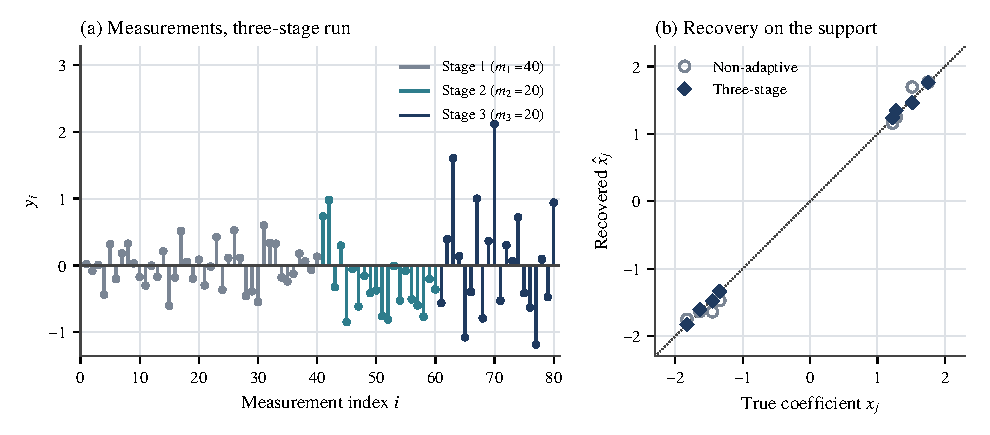
\includegraphics[width=\linewidth]{figures/measurements}
  \caption{\illus One run at $m=80$. (a) Measurements $y_i$ coloured by stage ($m_1,m_2,m_3=40,20,20$). (b) Recovered versus true coefficients on the support; the dotted line is perfect recovery.}\label{fig:measurements}
\end{figure}

% ===================================================================================================
\section{Discussion}\label{sec:discussion}
\textbf{RQ1.} Under an equal energy budget, concentrating sensing on a candidate support lowers the error by roughly half at $m=80$, and Eq.~\eqref{eq:var} explains the size of the effect through the energy gain in~\eqref{eq:energy}. \textbf{RQ2.} A second stage captures most of the gain and a third adds a further $20$--$30\%$ reduction at $m=64$--$80$, with diminishing returns beyond $m\approx100$ (Table~\ref{tab:sweep}); the oracle gap of about a factor three remains. \textbf{RQ3.} At $m=48$ the first stage has only $24$--$29$ measurements, too few to localise eight coefficients among $256$, and every non-oracle strategy fails (median error above $0.3$); adaptivity helped from $m=64$.

The trade-off is therefore between early information and late energy: a large first stage identifies the support reliably, a large last stage exploits it. This resembles distilled sensing~\cite{haupt2011} and Bayesian designs that direct measurements by posterior uncertainty~\cite{ji2008,chaloner1995}. The exact-recovery column of Table~\ref{tab:results} shows the price of discarding coordinates early: the two-stage design (first candidate set of $48$ coordinates) lowers the error but not the support-miss rate, whereas the three-stage design, whose first candidate set is wider ($64$), misses the support less often.

\section{Limitations}\label{sec:limits}
This is a simulation, not a study. The sparsity $s$ and the noise level $\sigma$ are known to the algorithm, amplitudes are bounded away from zero ($|x_j|\ge1$), which favours support estimation, and the signal is exactly sparse in the canonical basis. Stage sizes and candidate sizes were fixed in advance rather than optimised, and the gains are measured against one non-adaptive baseline only. The rows~\eqref{eq:rows} assume that arbitrary Gaussian combinations on a subset of coordinates can be realised in hardware. Re-solving the LASSO after every stage costs computation and latency. Finally, theory limits what adaptivity can achieve in general~\cite{ariascastro2013}, so the factors reported here must not be extrapolated to other noise levels, sparsity regimes or measurement models.

\section{Conclusion}\label{sec:conclusion}
We formulated budgeted multi-stage adaptive sampling for sparse recovery, gave a LASSO-based algorithm with an energy interpretation, and illustrated on synthetic data that three stages can roughly halve the median error of non-adaptive Gaussian sampling at $m=80$, while failing to help when the budget is too small to localise the support. Natural next steps are a data-driven choice of stage sizes, noise-adaptive regularisation, and validation on measured data.

% ---- Bibliography (inline: no .bib file needed). CUSTOMIZE: replace entries; keep keys in sync with \cite ----
\begin{thebibliography}{99}\small
\bibitem{candes2006} E.~J. Cand\`es, J.~Romberg and T.~Tao, ``Robust uncertainty principles: Exact signal reconstruction from highly incomplete frequency information,'' \emph{IEEE Trans. Inf. Theory}, vol.~52, no.~2, pp.~489--509, 2006.
\bibitem{donoho2006} D.~L. Donoho, ``Compressed sensing,'' \emph{IEEE Trans. Inf. Theory}, vol.~52, no.~4, pp.~1289--1306, 2006.
\bibitem{tibshirani1996} R.~Tibshirani, ``Regression shrinkage and selection via the lasso,'' \emph{J. R. Stat. Soc. Ser. B}, vol.~58, no.~1, pp.~267--288, 1996.
\bibitem{beck2009} A.~Beck and M.~Teboulle, ``A fast iterative shrinkage-thresholding algorithm for linear inverse problems,'' \emph{SIAM J. Imaging Sci.}, vol.~2, no.~1, pp.~183--202, 2009.
\bibitem{haupt2011} J.~Haupt, R.~M. Castro and R.~Nowak, ``Distilled sensing: Adaptive sampling for sparse detection and estimation,'' \emph{IEEE Trans. Inf. Theory}, vol.~57, no.~9, pp.~6222--6235, 2011.
\bibitem{ji2008} S.~Ji, Y.~Xue and L.~Carin, ``Bayesian compressive sensing,'' \emph{IEEE Trans. Signal Process.}, vol.~56, no.~6, pp.~2346--2356, 2008.
\bibitem{ariascastro2013} E.~Arias-Castro, E.~J. Cand\`es and M.~A. Davenport, ``On the fundamental limits of adaptive sensing,'' \emph{IEEE Trans. Inf. Theory}, vol.~59, no.~1, pp.~472--481, 2013.
\bibitem{chaloner1995} K.~Chaloner and I.~Verdinelli, ``Bayesian experimental design: A review,'' \emph{Statist. Sci.}, vol.~10, no.~3, pp.~273--304, 1995.
\bibitem{foucart2013} S.~Foucart and H.~Rauhut, \emph{A Mathematical Introduction to Compressive Sensing}. New York: Birkh\"auser, 2013.
\end{thebibliography}

\end{document}
